\chapter{Evaluation} \label{chapter:evaluation}
This chapter evaluates the malicious capabilities developed in our rootkit by comparing them to the original objectives we presented at the beginning of our research in Section \ref{section:project_objectives}. For this, we will analyse whether our rootkit meets the expected functionality by simulating a machine infection in a virtualized environment. A rootkit functionality will be considered fulfilled in the case it can be reproduced successfully in the experimental environment.

As we mentioned, the following are the functionalities we seeked to implement in our rootkit:
\begin{itemize}
\item Hijacking the execution of user programs while they are running, injecting libraries and executing malicious code, without impacting their normal execution.
\item Featuring a command-and-control module powered by a network backdoor, which can be operated from a remote client. This backdoor should be controlled with stealth in mind, featuring similar mechanisms to those present in rootkits found in the wild.
\item Tampering with user data at system calls, resulting in running malware-like programs and for other malicious purposes.
\item Achieving stealth, hiding rootkit-related files from the user.
\item Achieving rootkit persistence, the rootkit should run after a complete system reboot.
\end{itemize}

\section{Experimental setting}
The test environment that will be used to showcase the rootkit functionalities consists on two virtual machines running under Oracle VM VirtualBox \cite{virtualbox_page}. One of them will be the host infected with the rootkit, while the other will be used as the attacker machine from which to operate the rootkit client. 

Both virtual machines will be connected via a bridged adapter, as Figure \ref{fig:vm_setting_bridged} shows. With this virtual networking setting, the virtual machines connect to a device driver of the host system which injects the data received from the physical network \cite{bridged_networking}. From the virtual machine point of view, both the attacker and the infected machine appear to be physically connected (via a network cable) to the same network interface, each with a different assigned IP address. The name of this interface will be "enp0s3".

\begin{figure}[htbp]
	\centering
	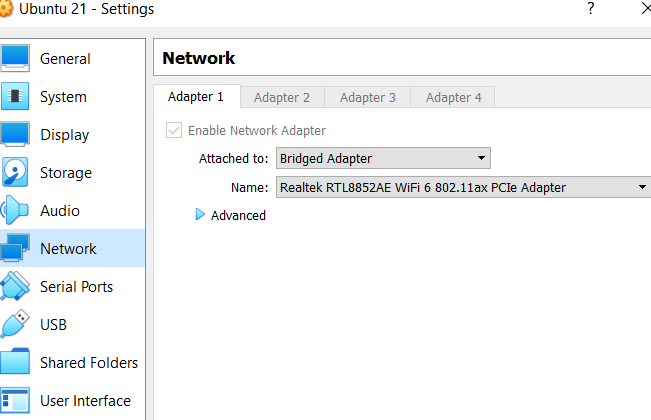
\includegraphics[width=13cm]{vm_setting_bridged.png}
	\caption{Network settings for both of the VMs on the test environment.}
	\label{fig:vm_setting_bridged}
\end{figure}

Table \ref{table:vm_config_test_environment} shows the role and charactersitics of the two machines. The overall test environment configuration with the described settings is illustrated in Figure \ref{fig:test_env}.

\begin{table}[H]
\begin{tabular}{|>{\centering\arraybackslash}p{3cm}|>{\centering\arraybackslash}p{3cm}|}
\hline
\multicolumn{2}{|c|}{\textbf{INFECTED MACHINE}}\\
\hline
\textbf{Attribute} & \textbf{Value}\\
\hline
\hline
User & osboxes\\
\hline
Operating System & GNU/Linux\\
\hline
Distribution & Ubuntu 21.04\\
\hline
Kernel version & 5.11.0-49\\
\hline
IP address & 192.168.1.124\\
\hline
\end{tabular}
\quad
\begin{tabular}{|>{\centering\arraybackslash}p{3cm}|>{\centering\arraybackslash}p{3cm}|}
\hline
\multicolumn{2}{|c|}{\textbf{ATTACKER MACHINE}}\\
\hline
\textbf{Attribute} & \textbf{Value}\\
\hline
\hline
User & RED\\
\hline
Operating System & GNU/Linux\\
\hline
Distribution & Ubuntu 18.04\\
\hline
Kernel version & 5.4.0-96\\
\hline
IP address & 192.168.1.127\\
\hline
\end{tabular}
\caption{Configuration of virtual machines in the test environment.}
\label{table:vm_config_test_environment}
\end{table}

\begin{figure}[htbp]
	\centering
	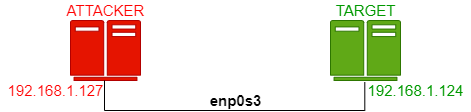
\includegraphics[width=13cm]{test_env.png}
	\caption{Network topology of test environment.}
	\label{fig:test_env}
\end{figure}



\section{Rootkit compilation and installation} \label{section:compile_install}
This section details the steps for a successful compilation and installation fo the rootkit in the target machine. Note that there also exist two scripts \textit{packager.sh} and \textit{deployer.sh} which automatize this process, but these are best indicated for an attacker which wants to quickly assemble the rootkit system, as we will explain in Section \ref{section:attack_scenario}.

\subsection{Compilation}
The rootkit source code incorporates two Makefile files that automatize the compilation process with the command \textit{make}. Table \ref{table:makefiles} details the location of the multiple Makefiles that must be executed to compile the different modules of the rootkit (note that in Section \ref{section:rootkit_arch} we described the rootkit files and their purpose in detail).

\begin{table}[htbp]
\begin{tabular}{|>{\centering\arraybackslash}p{2.2cm}|>{\centering\arraybackslash}p{2.2cm}|>{\centering\arraybackslash}p{4cm}|>{\centering\arraybackslash}p{4.5cm}|}
\hline
\textbf{MAKEFILE} & \textbf{COMMAND} &\textbf{DESCRIPTION}&\textbf{RESULT}\\
\hline
\hline
src/client/ Makefile & make & Compilation of the rootkit client & src/client/ injector\\
\hline
src/Makefile & make help & Compilation of programs for testing rootkit functionalities, and the malicious program and library of the execution hijacking and library injection modules respectively & src/helpers/simple\_timer, src/helpers/simple\_open, src/helpers/simple\_execve, src/helpers/lib\_injection.so, src/helpers/execve\_hijack\\
\hline
src/Makefile & make kit & Compilation of the rootkit using the libbpf library & src/bin/kit\\
\hline
src/Makefile & make tckit & Compilation of the rootkit TC egress program & src/bin/tc.o\\
\hline
\end{tabular}
\caption{Rootkit compilation Makefiles.}
\label{table:makefiles}
\end{table}

As we can observe in the table, there are two Makefiles:
\begin{itemize}
\item A Makefile under src/client to compile only the rootkit client.
\item A Makefile under src to compile all rootkit files.
\end{itemize}

Therefore, the complete compilation process would consist on the commands shown in Code snippet \ref{code:compilation}.
\begin{lstlisting}[language=C, caption={Rootkit and rootkit client compilation.}, label={code:compilation}]
//Rootkit files
cd src
make
//Rootkit client
cd client
make
\end{lstlisting}

The output programs corresponding to the rootkit will be stored under a directory \textit{src/bin}, while those belonging to helper and client programs will be stored together with the corresponding source code.

It must also be noted that, although the rootkit backdoor and C2 capabilities work out of the box, the rest of the rootkit modules need further configuration. This configuration is set via the src/common/constants.h file, and during the rest of this evaluation we will detail the relevant settings for each individual module.

\subsection{Installation}
Once the rootkit programs are compiled, the \textit{tc.o} and \textit{kit} programs must be loaded orderly. Code snippet \ref{code:installation} shows the commands to execute for installing the rootkit.

\begin{lstlisting}[language=C, caption={Rootkit installation steps.}, label={code:installation}]
//TC egress program
sudo tc qdisc add dev enp0s3 clsact
sudo tc filter add dev enp0s3 egress bpf direct-action obj bin/tc.o sec classifier/egress
//Libbpf-powered rootkit
sudo ./bin/kit -t enp0s3
\end{lstlisting}

Note that the network interface enp0s3 may be substituted with any other interface on which the attacker desires the backdoor to be operating.

Finally, we should create the files that guarantee the rootkit persistence, as shown in Code snippet \ref{code:persist}.
\begin{lstlisting}[language=C, caption={Creation of rootkit persistence files.}, label={code:persist}]
echo "* * * * * osboxes /bin/sudo /home/osboxes/TFG/src/helpers/deployer.sh" > /etc/cron.d/ebpfbackdoor
echo "osboxes ALL=(ALL:ALL) NOPASSWD:ALL #" > /etc/sudoers.d/ebpfbackdoor
\end{lstlisting}

The name of the user "osboxes" should be changed by that of the user of the machine to infect, together with the path on which the \textit{deployer.sh} script will be hidden.


\section{Attack scenario} \label{section:attack_scenario}
Although the steps presented in Section \ref{section:compile_install} were followed during the rootkit development, an attacker which has compromised a machine and wants to install the rootkit may benefit from a more automated process that quickly prepares all files and installs them in the target machine.

This section presents an hypothetical attack scenario, covering each of the steps the attacker must follow in order to prepare the rootkit and infect a machine:

A security researcher called 'RED' has managed to exploit a high-severity RCE vulnerability in a critical system controlled by an adversary which was found exposed to the Internet (e.g.: not behind a NAT \cite{nat_comptia}). After this exploitation, RED has now spawned a reverse shell connection with the privileged user 'osboxes', but he knows that the system is often rebooted and that he may lose access soon. Furthermore, the vulnerability he exploited is already well-known and may get patched in the near future, so he needs to persist his access. RED decides to load a classic rootkit consisting of a malicious kernel module, but he finds out that this capability is restricted in the system (e.g.: kernel.modules\_disabled=1 \cite{kernel_modules_restrict}), so he must find an alternative approach. Also, it is very possible that the system has an EDR logging events such as loading a kernel module (which almost assuredly will be considered by the EDR given that it is a very relevant event), so he needed to find a more stealthy path anyway. At some point, RED realises that even if kernel modules could not be used, the system administrator did not block eBPF, so he decides to use TripleCross.

Firstly, RED creates a secret directory where to hide the rootkit, and downloads it, as shown in Figure \ref{fig:post_exp}.

\begin{figure}[htbp]
	\centering
	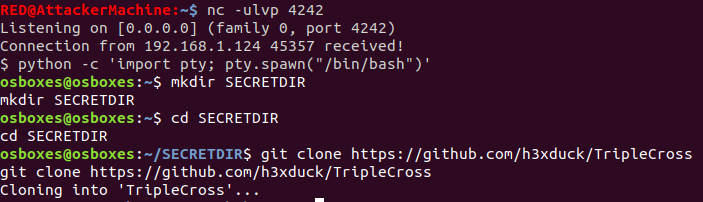
\includegraphics[width=13cm]{sch_post_exp.png}
	\caption{Creation of hidden directory and downloading rootkit.}
	\label{fig:post_exp}
\end{figure}

Once it is downloaded, RED executes the \textit{packager.sh} script, that will compile the rootkit. Alternatively, an attacker could have compiled it locally and sent it to the remote machine afterwards.

After the script execution finishes, a folder \textit{apps} has been generated with all the rootkit files. This directory contains all the files and scripts needed for the rootkit installation. RED now executes the \textit{deployer.sh} script, which installs the rootkit and writes the persistence files, as shown in Figure \ref{fig:deploy_root}

\begin{figure}[htbp]
	\centering
	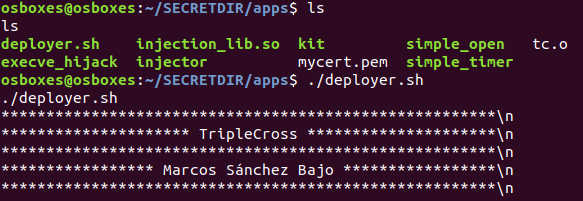
\includegraphics[width=13cm]{sch_deploy_root.png}
	\caption{Files created by packager.sh and execution of deployer.sh.}
	\label{fig:deploy_root}
\end{figure}

Once the script has been executed, all rootkit modules are loaded and the backdoor is already waiting for commands. RED can now close the reverse shell and open the rootkit client. He now has persistent privileged access to the infected machine.

\section{Hijacking execution of running processes}
Following the infection process described in Section \ref{section:attack_scenario}, The rootkit can hijack the execution of running processes by means of the library injection module. This module incorporates two sample programs (\textit{src/helpers/simple\_timer.c and src/helpers/simple\_open.c}), both containing the execution of one of the hijacked syscalls (sys\_timerfd\_settime and sys\_openat respectively). Additionally, the functionality can be tested in any process of the infected machine by changing its settings. Table \ref{table:lib_injection_config} shows how to customize the functionality of the library injection module.

\begin{table}[htbp]
\begin{tabular}{|>{\centering\arraybackslash}p{2.8cm}|>{\centering\arraybackslash}p{5.2cm}|>{\centering\arraybackslash}p{5.2cm}|}
\hline
\textbf{FILENAME} & \textbf{CONSTANT} & \textbf{DESCRIPTION}\\
\hline
\hline
src/common/ constants.h & TASK\_COMM\_NAME\_INJECTION\_TARGET\_TIMERFD\_SETTIME & Name of process to hijack at syscall sys\_timerfd\_settime.\\
\hline
src/common/ constants.h & TASK\_COMM\_NAME\_INJECTION\_TARGET\_OPEN & Name of process to hijack at syscall sys\_openat.\\
\hline
src/helpers/ injection\_lib.c & ATTACKER\_IP \& ATTACKER\_PORT & IP address and port of attacker machine\\
\hline
\end{tabular}
\caption{Library injection module configuration.}
\label{table:lib_injection_config}
\end{table}

After a successful injection the malicious library will run a reverse shell against the attacker machine. Also, it will print a message for us to check it locally. Therefore, from the attacker machine, we will listen to the specified IP and port, considering the injection successful if a connection is opened.


\subsection{Test program simple\_timer}
Table \ref{table:lib_injection_config_simple_timer} shows the module configuration for running this attack.

\begin{table}[htbp]
\begin{tabular}{|>{\centering\arraybackslash}p{3cm}|>{\centering\arraybackslash}p{5.5cm}|>{\centering\arraybackslash}p{4cm}|}
\hline
\textbf{FILENAME} & \textbf{CONSTANT} & \textbf{VALUE}\\
\hline
\hline
src/common/ constants.h & TASK\_COMM\_NAME\_INJECTION\_TARGET\_TIMERFD\_SETTIME & "simple\_timer"\\
\hline
src/helpers/ injection\_lib.c & ATTACKER\_IP \& ATTACKER\_PORT & 192.168.1.127 \& 5555 \\
\hline
\end{tabular}
\caption{Library injection module configuration for attacking simple\_timer.c.}
\label{table:lib_injection_config_simple_timer}
\end{table}

Figure \ref{fig:sc_lib_inj_simple_timer_off} shows the execution of the simple\_timer process without the rootkit installed.

\begin{figure}[htbp]
	\centering
	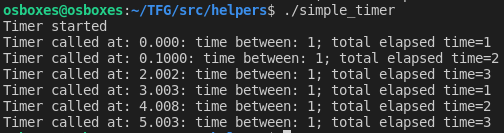
\includegraphics[width=13cm]{sch_sc_lib_inj_simple_timer_off.png}
	\caption{Normal execution of simple\_timer program.}
	\label{fig:sc_lib_inj_simple_timer_off}
\end{figure}

Once the rootkit is installed it starts the module automatically, looking for system calls from the simple\_timer process.
The attacker must in the mean time start a listener (e.g.: with netcat), as shown in Figure \ref{fig:sc_lib_inj_nc}.

\begin{figure}[htbp]
	\centering
	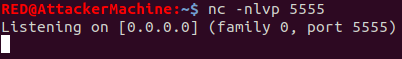
\includegraphics[width=12cm]{sch_sc_lib_inj_nc.png}
	\caption{Attacker waiting for a connection with netcat.}
	\label{fig:sc_lib_inj_nc}
\end{figure}

Then, the simple\_timer program gets executed on the infected machine. As we can observe in Figure \ref{fig:sc_lib_inj_simple_timer_exec}, the injection suceeds and a message is printed from the library. 

\begin{figure}[htbp]
	\centering
	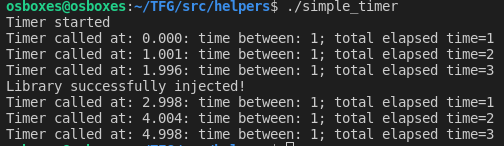
\includegraphics[width=12cm]{sch_sc_lib_inj_simple_timer_exec.png}
	\caption{Execution of simple\_timer.c with rootkit active.}
	\label{fig:sc_lib_inj_simple_timer_exec}
\end{figure}


Figure \ref{fig:sc_lib_inj_nc_success} shows the attacker connected to the reverse shell launched from the library.

\begin{figure}[htbp]
	\centering
	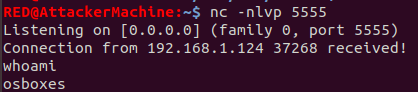
\includegraphics[width=12cm]{sch_sc_lib_inj_nc_success.png}
	\caption{Reverse shell received after library injection attack.}
	\label{fig:sc_lib_inj_nc_success}
\end{figure}


\subsection{Test program simple\_open}
The library injection module can also be tested with the simple\_timer program, which opens multiple files with sys\_openat. The rootkit configuration for this is shown in Table \ref{table:lib_injection_config_simple_open}.

\begin{table}[htbp]
\begin{tabular}{|>{\centering\arraybackslash}p{3cm}|>{\centering\arraybackslash}p{5.2cm}|>{\centering\arraybackslash}p{4cm}|}
\hline
\textbf{FILENAME} & \textbf{CONSTANT} & \textbf{VALUE}\\
\hline
\hline
src/common/ constants.h & TASK\_COMM\_NAME\_INJECTION\_TARGET\_OPEN & "simple\_open"\\
\hline
src/helpers/ injection\_lib.c & ATTACKER\_IP \& ATTACKER\_PORT & 192.168.1.127 \& 5555 \\
\hline
\end{tabular}
\caption{Library injection module configuration for attacking simple\_open.c.}
\label{table:lib_injection_config_simple_open}
\end{table}

As we can observe in figure \ref{fig:sc_lib_inj_simple_open}, when the injection suceeds, a message is printed on screen. Also, the attacker receives a shell, like we showed in Figure \ref{fig:sc_lib_inj_nc_success}.

\begin{figure}[htbp]
	\centering
	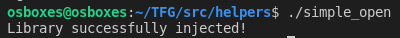
\includegraphics[width=12cm]{sch_sc_lib_inj_simple_open.png}
	\caption{Execution of simple\_open with rootkit active.}
	\label{fig:sc_lib_inj_simple_open}
\end{figure}


\subsection{Hijacking systemd}
Apart from the test programs, the library injection module can also inject the malicious library on any process of the system that makes use of either sys\_openat or sys\_timerfd\_settime. By hijacking privileged system programs such as systemd, the malicious library can achieve automatic root permissions once it is run (although these are anyways automatically granted via the privilege escalation module). Table \ref{table:lib_injection_config_systemd} shows the module configuration for running an attack against this process.

\begin{table}[htbp]
\begin{tabular}{|>{\centering\arraybackslash}p{3cm}|>{\centering\arraybackslash}p{5.5cm}|>{\centering\arraybackslash}p{4cm}|}
\hline
\textbf{FILENAME} & \textbf{CONSTANT} & \textbf{VALUE}\\
\hline
\hline
src/common/ constants.h & TASK\_COMM\_NAME\_INJECTION\_TARGET\_TIMERFD\_SETTIME & "systemd"\\
\hline
src/common/ constants.h & TASK\_COMM\_NAME\_INJECTION\_TARGET\_OPEN & "systemd"\\
\hline
src/helpers/ injection\_lib.c & ATTACKER\_IP \& ATTACKER\_PORT & 192.168.1.127 \& 5555 \\
\hline
\end{tabular}
\caption{Library injection module configuration for attacking the systemd process.}
\label{table:lib_injection_config_systemd}
\end{table}

With these configurations, we can run the rootkit and wait for systemd to call one of these syscalls. Eventually this call occurs, and using the debug messages of the rootkit we can get information on what happened, as shown in Figure \ref{fig:sc_lib_inj_systemd_debug}.

\begin{figure}[htbp]
	\centering
	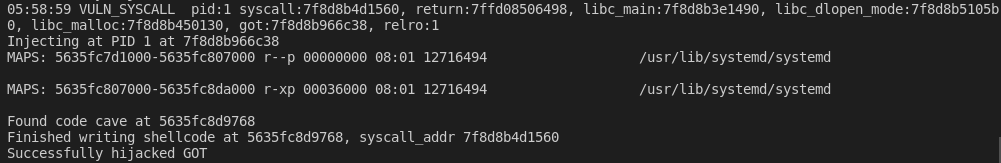
\includegraphics[width=12cm]{sch_sc_lib_inj_systemd_debug.png}
	\caption{Rootkit debug messages showing library injection.}
	\label{fig:sc_lib_inj_systemd_debug}
\end{figure}

As we can observe in the figure, the rootkit finds the relevant addresses via the technique we described on Section \ref{section:lib_injection} and proceeds to overwrite the GOT address. The library is loaded and executed, and since systemd is executed by the root user, the attacker receives a root shell as shown in Figure \ref{fig:lib_inj_success_root}. Most importantly, the systemd process does not crash after this attack.

\begin{figure}[htbp]
	\centering
	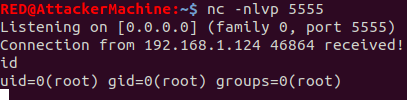
\includegraphics[width=12cm]{sch_lib_inj_success_root.png}
	\caption{Reverse shell received with root user after systemd library injection.}
	\label{fig:lib_inj_success_root}
\end{figure}


\section{Backdoor and C2}
The backdoor module works out of the box without any additional configurations needed. It includes the C2 capabilities and the rootkit client used to communicate with the backdoor. As we described in Section \ref{subsection:rootkit_manual}, the client allows for the operations listed on Table \ref{table:rootkit_client_actions}.

\begin{table}[htbp]
\begin{tabular}{|>{\centering\arraybackslash}p{5cm}|>{\centering\arraybackslash}p{8.5cm}|}
\hline
\textbf{PROGRAM ARGUMENTS} & \textbf{ACTION DESCRIPTION}\\
\hline
\hline
./injector -c <Victim IP> & Spawns a plaintext pseudo-shell by using the execution hijacking module.\\
\hline
./injector -e <Victim IP> & Spawns an encrypted pseudo-shell by commanding the backdoor with a pattern-based trigger.\\
\hline
./injector -s <Victim IP> & Spawns an encrypted pseudo-shell by commanding the backdoor with a multi-packet trigger (of both types).\\
\hline
./injector -p <Victim IP> & Spawns a phantom shell by commanding the backdoor with a pattern-based trigger.\\
\hline
./injector -a <Victim IP> & Orders the rootkit to activate all eBPF programs.\\
\hline
./injector -a <Victim IP> & Orders the rootkit to detach all of its eBPF programs.\\
\hline
./injector -S <Victim IP> & Showcases how the backdoor can hide a message from the kernel.\\
\hline
./injector -h & Displays help.\\
\hline
\end{tabular}
\caption{Rootkit client options.}
\label{table:rootkit_client_actions}
\end{table}

Once the rootkit is installed, the backdoor is launched automatically and will wait for backdoor triggers ready to launch the corresponding requested actions.

\subsection{Spawning encrypted pseudo-shells}
Encrypted pseudo-shells can be spawned using the rootkit client either with pattern-based or multi-packet backdoor triggers.

\textbf{Pattern-based triggers}\\
When using a pattern-based trigger, the attacker must indicate the following information:
\begin{itemize}
\item The IP address of the infected machine.
\item The network interface to use for sending the trigger.
\end{itemize}

As Figure \ref{fig:sc_eps_rc} shows, the backdoor executes the requested action and starts an encrypted pseudo-shell connection with privileged permissions in which the attacker can introduce commands to be executed. Whenever the connection shall be closed, the attacker introduces the "EXIT" global command (as we explained in Section \ref{subsection:rootkit_manual}), which ends the transmission gracefully.

\begin{figure}[htbp]
	\centering
	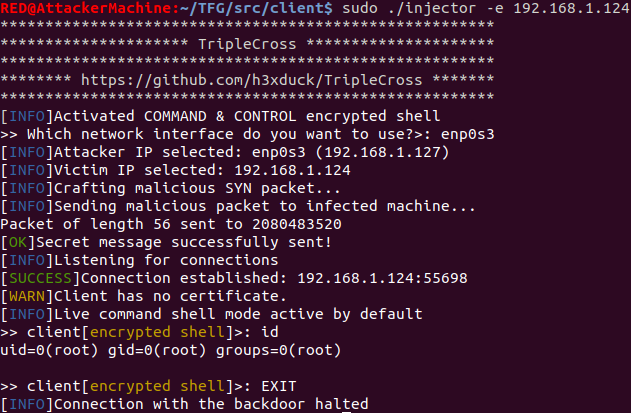
\includegraphics[width=12cm]{sch_sc_eps_rc.png}
	\caption{Encrypted pseudo-shell with rootkit client using pattern-based trigger.}
	\label{fig:sc_eps_rc}
\end{figure}

\textbf{Multi-packet triggers}\\
The rootkit client offers multiple options when using the multi-packet backdoor triggers. In particular, the attacker must specify the following fields:
\begin{itemize}
\item The IP address of the infected machine.
\item The network interface to use for sending the trigger.
\item Whether to hide the payload at the TCP sequence numbers or at the TCP source port.
\end{itemize}

Figure \ref{fig:sc_eps_seqnum} shows how the rootkit client asks for this data and spawns an encrypted pseudo-shell with the client when hiding the payload at the TCP sequence number. As we can observe in the figure, the payload is divided in 3 different chunks and injected to a stream of packets, which are sent in an orderly manner.

\begin{figure}[htbp]
	\centering
	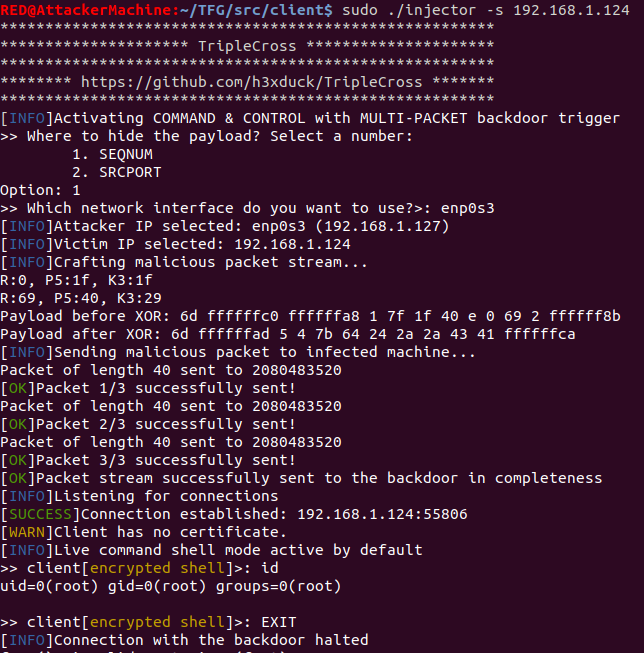
\includegraphics[width=12cm]{sch_sc_eps_seqnum.png}
	\caption{Encrypted pseudo-shell with rootkit client using multi-packet trigger with payload hidden in TCP sequence number.}
	\label{fig:sc_eps_seqnum}
\end{figure}

Figure \ref{fig:sc_eps_srcport} shows the same process but using the TCP source port as a means for hiding the data payload. As we can observe in the figure, in this case the paylaod is divided in 6 chunks.

\begin{figure}[htbp]
	\centering
	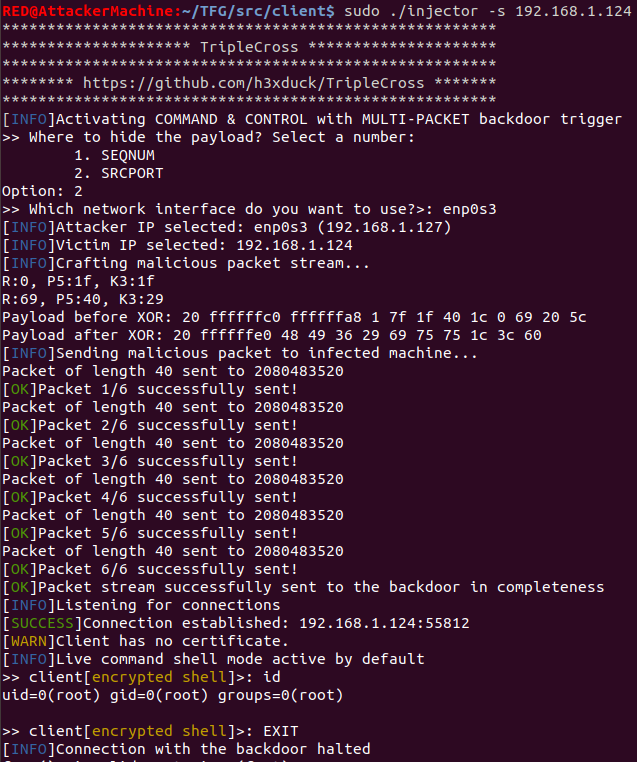
\includegraphics[width=12cm]{sch_sc_eps_srcport.png}
	\caption{Encrypted pseudo-shell with rootkit client using multi-packet trigger with payload hidden in TCP source port.}
	\label{fig:sc_eps_srcport}
\end{figure}

\subsection{Spawning phantom shells}
A phantom shell can be spawned using the rootkit client by sending pattern-based backdoor triggers. As we explained in Section \ref{subsection:c2}, the response to a client command will only be received once a TCP packet is sent from the infected machine to some location. Therefore, we need to wait until any application sends a TCP packet.

For requesting a phantom shell, the attacker must introduce the following arguments:
\begin{itemize}
\item The IP address of the infected machine.
\item The network interface to use for sending the trigger.
\end{itemize}

Once the request is sent by the rootkit client, it will scan the network for the response. As Figure \ref{fig:sc_phantom_1} shows, this rootkit client displays an alert whenever a packet is received.

\begin{figure}[htbp]
	\centering
	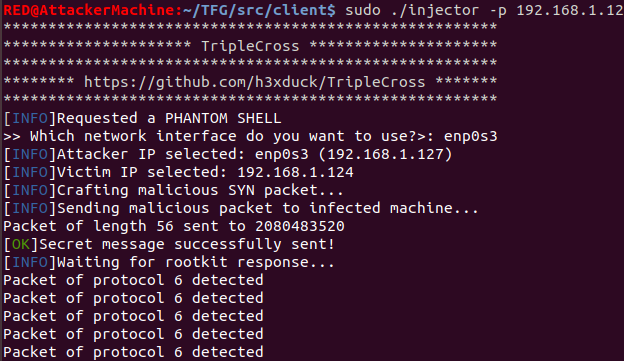
\includegraphics[width=12cm]{sch_sc_phantom_1.png}
	\caption{Requesting a phantom shell with the rootkit client.}
	\label{fig:sc_phantom_1}
\end{figure}

At some point, the infected machine will send a TCP packet to any host. We can speed up this process by, for instance, launching a web broswer and visiting any page. When this happens, one TCP packet will be hijacked and sent to the rootkit client, which will show the attacker that the phantom shell is now ready to introduce commands, as shown in figure \ref{fig:sc_phantom_2}.

\begin{figure}[htbp]
	\centering
	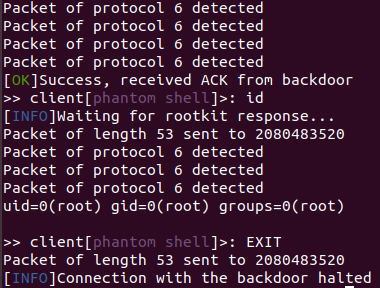
\includegraphics[width=11cm]{sch_sc_phantom_2.png}
	\caption{Rootkit client after phantom shell response is received.}
	\label{fig:sc_phantom_2}
\end{figure}



\subsection{eBPF programs control}
The rootkit client incorporates two commands to operate the state of the rootkit eBPF programs using the backdoor, enabling to activate or deactivate them as a group.

Figure \ref{fig:sc_unload_rc} shows how the attacker can detach all eBPF programs (except the backdoor, which as we mentioned in Section \ref{subsection:c2} must stay attached to receive further commands).

\begin{figure}[htbp]
	\centering
	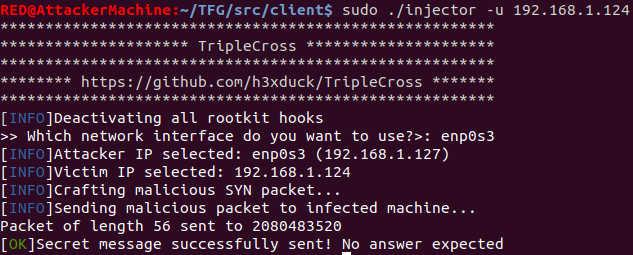
\includegraphics[width=12cm]{sch_sc_unload_rc.png}
	\caption{Requesting to detach all eBPF programs using rootkit client.}
	\label{fig:sc_unload_rc}
\end{figure}

Once the command is executed, we can check that, for instance, the privilege execution module is unloaded, as shown in Figure \ref{fig:sc_unload_res}.

\begin{figure}[htbp]
	\centering
	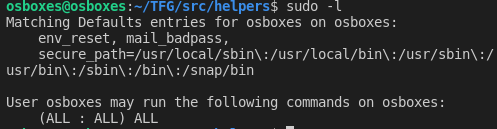
\includegraphics[width=12cm]{sch_sc_unload_res.png}
	\caption{User osboxes permissions after eBPF programs are detached.}
	\label{fig:sc_unload_res}
\end{figure}

Since the backdoor will be still running, the attacker can now request to attach all eBPF programs again, as shown in Figure \ref{fig:sc_attach_rc}

\begin{figure}[htbp]
	\centering
	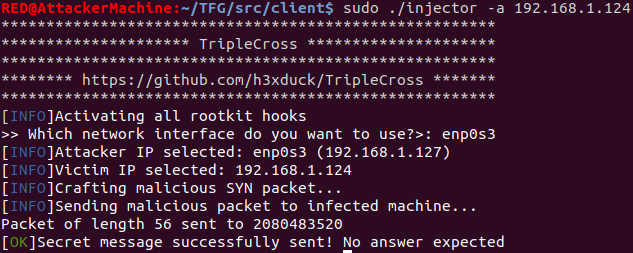
\includegraphics[width=12cm]{sch_sc_attach_rc.png}
	\caption{Requesting to attach all eBPF programs using rootkit client.}
	\label{fig:sc_attach_rc}
\end{figure}

After the command is executed, all rootkit modules will be loaded again. We can check it by observing the permissions of the user osboxes, as shown in Figure \ref{fig:sc_attach}.

\begin{figure}[htbp]
	\centering
	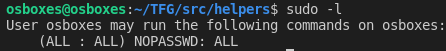
\includegraphics[width=12cm]{sch_sc_attach.png}
	\caption{User osboxes permissions after eBPF programs are attached.}
	\label{fig:sc_attach}
\end{figure}


\subsection{Modifying incoming traffic (PoC)} \label{subsection:poc_evaluation}
The backdoor incorporates a simple proof of concept to show how the rootkit may modify incoming network traffic. Although this feature has not been integrated in any of the C2 modules, we considered this functionality to be relevant enough to implement it individually.

This PoC shows the rootkit client sending a packet with a payload \textit{"XDP\_PoC\_0"} sent to the infected machine port 9000. Upon inspection of this packet, the machine will read the content as \textit{"The previous message has been hidden"}. Figure \ref{fig:sc_poc_rc} shows how the rootkit client can send this packet.

\begin{figure}[htbp]
	\centering
	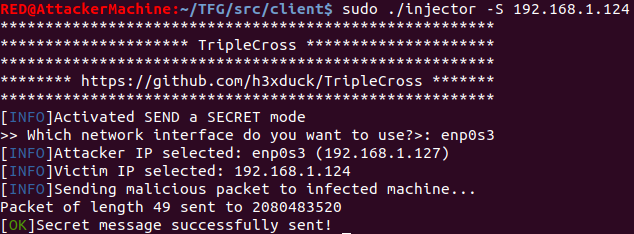
\includegraphics[width=12cm]{sch_sc_poc_rc.png}
	\caption{Sending packet for traffic modification PoC with rootkit client.}
	\label{fig:sc_poc_rc}
\end{figure}

To perform this PoC we will use tcpdump (which we explained in Section \ref{subsection:tcpdump}) to inspect the received packets. Figure \ref{fig:sc_tcpdump_before} shows the packet and payload received when the rootkit is not installed.

\begin{figure}[htbp]
	\centering
	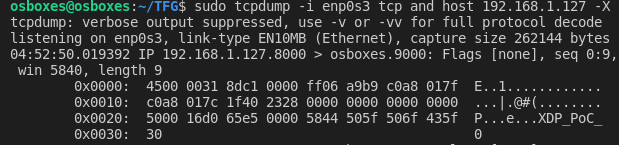
\includegraphics[width=12cm]{sch_tcpdump_before.png}
	\caption{Packet captured with tcpdump in traffic modification PoC with rootkit not installed.}
	\label{fig:sc_tcpdump_before}
\end{figure}

Once the rootkit is installed, it will modify the length and contents, as shown in Figure \ref{fig:sc_tcpdump_after}.

\begin{figure}[htbp]
	\centering
	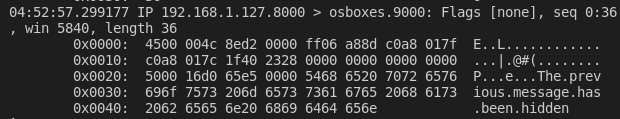
\includegraphics[width=12cm]{sch_tcpdump_after.png}
	\caption{Packet captured with tcpdump in traffic modification PoC with rootkit installed.}
	\label{fig:sc_tcpdump_after}
\end{figure}


\section{Tampering with system calls}
This functionality has been incorporated in multiple rootkit modules, but it is particularly relevant in the execution hijacking and privilege escalation modules.

\subsection{Hijacking programs execution}
Once the rootkit is installed, it will attempt to hijack any new program that is executed. As we explained in Section \ref{section:execution_hijack}, once the rootkit suceeds a malicious program will be run, which will listen for commands from the rootkit client, enabling the attacker to open a plaintext pseudo-shell. 

In this evaluation, we will attempt to test the hijacking process with a test program \textit{src/helpers/simple\_execve} and another with any process of the machine. Table \ref{table:execution_hijack_config} shows some of the configuration options that must be selected before running this module.

\begin{table}[htbp]
\begin{tabular}{|>{\centering\arraybackslash}p{3cm}|>{\centering\arraybackslash}p{4.5cm}|>{\centering\arraybackslash}p{6cm}|}
\hline
\textbf{FILENAME} & \textbf{CONSTANT} & \textbf{DESCRIPTION}\\
\hline
\hline
src/common/ constants.h & PATH\_EXECUTION\_HIJACK\_PROGRAM & Location of the malicious program to be executed upon succeeding to execute a sys\_execve call.\\
\hline
src/common/ constants.h & EXEC\_HIJACK\_ACTIVE & Deactivate (0) or activate (1) the execution hijacking module.\\
\hline
src/common/ constants.h & TASK\_COMM\_RESTRICT\_HIJACK\_ACTIVE  & Hijack any sys\_execve call (0) or only those indicated in TASK\_COMM\_NAME\_RESTRICT\_HIJACK (1).\\
\hline
src/common/ constants.h & TASK\_COMM\_NAME\_RESTRICT\_HIJACK & Name of the program from which to hijack sys\_execve calls.\\
\hline
\end{tabular}
\caption{Execution hijacking module configuration.}
\label{table:execution_hijack_config}
\end{table}


\textbf{Test program simple\_execve}\\
This program contains a simple sys\_execve call that runs the bash command "pwd", which displays the current directory. As we can observe in Table \ref{table:execution_hijack_config_simple_execve}, for this test we will set the PATH\_EXECUTION\_HIJACK\_PROGRAM setting to the path where we have hidden the malicious program, and set the TASK\_COMM\_NAME\_RESTRICT\_HIJACK setting to indicate that we want to hijack calls executed from the simple\_execve program.

\begin{table}[htbp]
\begin{tabular}{|>{\centering\arraybackslash}p{3cm}|>{\centering\arraybackslash}p{4.5cm}|>{\centering\arraybackslash}p{4cm}|}
\hline
\textbf{FILENAME} & \textbf{CONSTANT} & \textbf{VALUE}\\
\hline
\hline
src/common/ constants.h & PATH\_EXECUTION\_HIJACK\_PROGRAM & "/home/osboxes/ SECRETDIR/ src/helpers/ execve\_hijack"\\
\hline
src/common/ constants.h & EXEC\_HIJACK\_ACTIVE & 1\\
\hline
src/common/ constants.h & TASK\_COMM\_RESTRICT\_HIJACK\_ACTIVE & 1\\
\hline
src/common/ constants.h & TASK\_COMM\_NAME\_RESTRICT\_HIJACK & "simple\_execve"\\
\hline
\end{tabular}
\caption{Execution hijacking module configuration for attacking test program simple\_execve.}
\label{table:execution_hijack_config_simple_execve}
\end{table}

Figure \ref{fig:sc_execve_hijack_before_simple_execve} shows the normal execution of the simple\_execve program. As we can observe, it prints the current directory, as expected.

\begin{figure}[htbp]
	\centering
	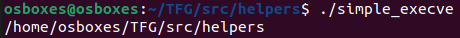
\includegraphics[width=12cm]{sch_sc_execve_hijack_before.png}
	\caption{Execution of test program simple\_execve with rootkit not installed.}
	\label{fig:sc_execve_hijack_before_simple_execve}
\end{figure}

Once the rootkit is installed, we will open a shell in the infected machine and execute again the simple\_execve program. The result is shown in Figure \ref{fig:sc_execve_hijack_simple_execve}.

\begin{figure}[htbp]
	\centering
	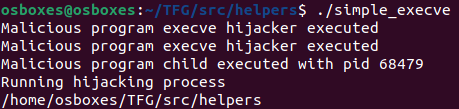
\includegraphics[width=12cm]{sch_sc_execve_hijack.png}
	\caption{Execution of test program simple\_execve with rootkit installed.}
	\label{fig:sc_execve_hijack_simple_execve}
\end{figure}

As we can observe in the figure, the rootkit hijacked the call and executed the malicious program instead. Each time the malicious program is executed, it alerts us with a message (this would be hidden in a non-experimental case). We can see that it is executed twice (since it needs to run itself as sudo, as we explained in Section \ref{subsection:hijack_program_exec}) and then it forks() itself and executes the original program (we can see the output of pwd) and then starts to listen for the rootkit client connections. Figure \ref{fig:sc_execution_hijack_simple_execve_rc} shows how the rootkit client spawns a plaintext pseudo-shell with the malicious program and runs a command.

\begin{figure}[htbp]
	\centering
	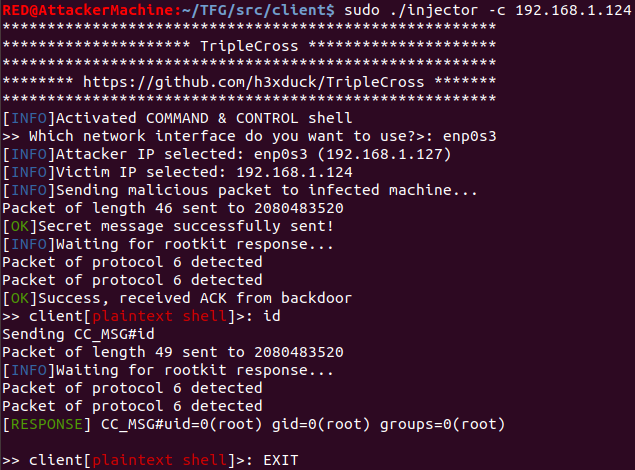
\includegraphics[width=13cm]{sch_sc_execution_hijack_simple_execve_rc.png}
	\caption{Spawning plaintext pseudo-shell with rootkit client.}
	\label{fig:sc_execution_hijack_simple_execve_rc}
\end{figure}

As we can observe in the figure, the rootkit client will connect to the malicious program, enabling the attacker to send any command. Once it is received by the malicious program, it will execute it and answer back to the rootkit client with the output according to the plaintext pseudo-shell network protocol. As shown in Figure \ref{fig:sc_execution_hijack_im}, the malicious program shows information about the actions that have been executed (which would be hidden in a real scenario).

\begin{figure}[htbp]
	\centering
	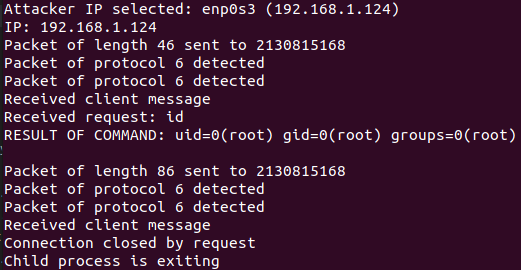
\includegraphics[width=13cm]{sch_sc_execution_hijack_im.png}
	\caption{Execition of command requested from rootkit client in the infected machine.}
	\label{fig:sc_execution_hijack_im}
\end{figure}


\textbf{Hijacking the execution of any program}\\
As we mentioned in Section \ref{section:execution_hijack}, it is possible that programs fail to be hijacked due to page faults. Because of this, it can take a long time for an specific program (such as bash) to trigger the execution of the malicious program so that the attacker can connect via the plaintext pseudo-shell. This is the reason why the rootkit can also be set to attempt hijacking any program execution from the system instead of restricting the operation to a single process. In this mode, the rootkit will attempt to hijack any sys\_execve call until it succeeds once, afterwards the execution hijacking module will be deactivated. Table \ref{table:execution_hijack_config_any} shows the configuration for this mode.

\begin{table}[htbp]
\begin{tabular}{|>{\centering\arraybackslash}p{3cm}|>{\centering\arraybackslash}p{4.5cm}|>{\centering\arraybackslash}p{4cm}|}
\hline
\textbf{FILENAME} & \textbf{CONSTANT} & \textbf{VALUE}\\
\hline
\hline
src/common/ constants.h & PATH\_EXECUTION\_HIJACK\_PROGRAM & "/home/osboxes/ SECRETDIR/ src/helpers/execve\_hijack"\\
\hline
src/common/ constants.h & EXEC\_HIJACK\_ACTIVE & 1\\
\hline
src/common/ constants.h & TASK\_COMM\_RESTRICT\_HIJACK\_ACTIVE & 0\\
\hline
src/common/ constants.h & TASK\_COMM\_NAME\_RESTRICT\_HIJACK & ""\\
\hline
\end{tabular}
\caption{Execution hijacking module configuration for attempting to hijack any sys\_execve call.}
\label{table:execution_hijack_config_any}
\end{table}

The process will be identical to that shown with the test program simple\_execve. Once a sys\_execve call is hijacked, the malicious program will listen for comamnds sent from the rootkit client, as we showed previously in Figure \ref{fig:sc_execution_hijack_simple_execve_rc}.


\subsection{Privilege escalation}
As we showed in Section \ref{section:privesc}, the privilege escalation module tampers with system calls buffers to modify the contents read from the \textit{/etc/sudoers} file by the sudo process. Figure \ref{fig:sc_sudo_prev} shows the sudo permissions of user osboxes previously to the installation of the rootkit. As we can observe, it has sudo privileges, but requires a password.

\begin{figure}[htbp]
	\centering
	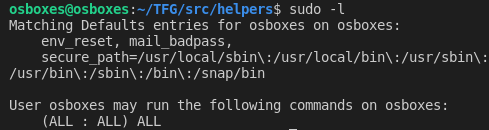
\includegraphics[width=12cm]{sch_sc_sudo_prev.png}
	\caption{Sudo privileges of user osboxes before rootkit installation.}
	\label{fig:sc_sudo_prev}
\end{figure}

Once the rootkit is installed, every time the sudo process requests to read the \textit{/etc/sudoers} file, the contents will be modified. Figure \ref{fig:sc_sudo_after} shows that now the user osboxes appears to have sudo privileges without requiring a password.

\begin{figure}[htbp]
	\centering
	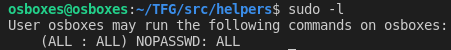
\includegraphics[width=12cm]{sch_sc_sudo_after.png}
	\caption{Sudo privileges of user osboxes after rootkit installation.}
	\label{fig:sc_sudo_after}
\end{figure}

Note that this modification only applies to the sudo process. For instance, if any user wants to read the \textit{/etc/sudoers} file, it appears intact as shown in Figure \ref{fig:sc_sudoers}.

\begin{figure}[htbp]
	\centering
	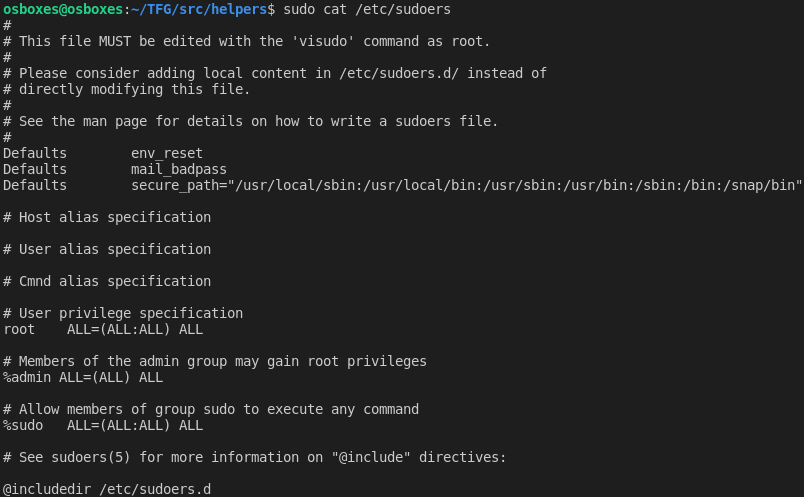
\includegraphics[width=12cm]{sch_sc_sudoers.png}
	\caption{Reading sudoers file after rootkit installation.}
	\label{fig:sc_sudoers}
\end{figure}

\subsection{Rootkit stealth}
As we presented in Section \ref{section:rootkti_stealth}, the following files and directories will be hidden by the rootkit:
\begin{itemize}
\item Files named "ebpfbackdoor", to hide those corresponding to the rootkit persistence.
\item Entire directories named "SECRETDIR", to hide the rootkit files.
\end{itemize}

The files and directories being hidden can be modified by using the settings shown in Table \ref{table:rootkit_stealth_config}.

\begin{table}[htbp]
\begin{tabular}{|>{\centering\arraybackslash}p{3cm}|>{\centering\arraybackslash}p{4.5cm}|>{\centering\arraybackslash}p{6cm}|}
\hline
\textbf{FILENAME} & \textbf{CONSTANT} & \textbf{DESCRIPTION}\\
\hline
\hline
src/common/ constants.h & SECRET\_DIRECTORY\_NAME\_HIDE & Name of directory to hide.\\
\hline
src/common/ constants.h & SECRET\_FILE\_PERSISTENCE\_NAME & Name of the file to hide.\\
\hline
\end{tabular}
\caption{Rootkit stealth module configuration.}
\label{table:rootkit_stealth_config}
\end{table}

We will now test this module in the infected machine.

\textbf{Hiding rootkit directory}\\
In the attack scenario we described in Section \ref{section:attack_scenario}, the SECRETDIR directory was created under \textit{/home/osboxes} and it was set as the root directory where to hide the rootkit files. Table \ref{table:rootkit_stealth_config_dir} details the rootkit configuration needed to hide this directory.

\begin{table}[htbp]
\begin{tabular}{|>{\centering\arraybackslash}p{3cm}|>{\centering\arraybackslash}p{4.5cm}|>{\centering\arraybackslash}p{6cm}|}
\hline
\textbf{FILENAME} & \textbf{CONSTANT} & \textbf{VALUE}\\
\hline
\hline
src/common/ constants.h & SECRET\_DIRECTORY\_NAME\_HIDE & "SECRETDIR"\\
\hline
\end{tabular}
\caption{Rootkit configuration for hiding directory "SECRETDIR".}
\label{table:rootkit_stealth_config_dir}
\end{table}

Listing the files and directories under the command \textit{ls} yields the results shown in Figure \ref{fig:sc_stealth_dir_before}.

\begin{figure}[htbp]
	\centering
	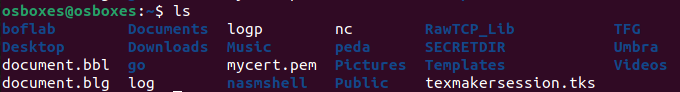
\includegraphics[width=13cm]{sch_sc_stealth_dir_before.png}
	\caption{Listing files and directories at the home directory before rootkit installation.}
	\label{fig:sc_stealth_dir_before}
\end{figure}

After the rootkit is loaded, we can observe in Figure \ref{fig:sc_stealth_dir_after} that the directory SECRETDIR is not visible anymore.

\begin{figure}[htbp]
	\centering
	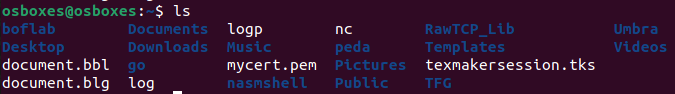
\includegraphics[width=13cm]{sch_sc_stealth_dir_after.png}
	\caption{Listing files and directories at the home directory after rootkit installation.}
	\label{fig:sc_stealth_dir_after}
\end{figure}

\textbf{Hiding persistence files}\\
Hiding the \textit{ebpfbackdoor} files can be achieved using the configuration shown in Table \ref{table:rootkit_stealth_config_file}.

\begin{table}[htbp]
\begin{tabular}{|>{\centering\arraybackslash}p{3cm}|>{\centering\arraybackslash}p{4.5cm}|>{\centering\arraybackslash}p{6cm}|}
\hline
\textbf{FILENAME} & \textbf{CONSTANT} & \textbf{VALUE}\\
\hline
\hline
src/common/ constants.h & SECRET\_FILE\_PERSISTENCE\_NAME & "ebpfbackdoor"\\
\hline
\end{tabular}
\caption{Rootkit configuration for hiding file "ebpfbackdoor".}
\label{table:rootkit_stealth_config_file}
\end{table}

As we can observe in Figure \ref{fig:sc_stealth_file_before}, this file is visible before installing the backdoor.

\begin{figure}[htbp]
	\centering
	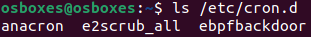
\includegraphics[width=12cm]{sch_sc_stealth_file_before.png}
	\caption{Listing files and directories at the cron.d directory before rootkit installation.}
	\label{fig:sc_stealth_file_before}
\end{figure}

However, once the rootkit is installed, the file will not be listed under the directory (or any other), as shown in Figure \ref{fig:sc_stealth_file_after}.

\begin{figure}[htbp]
	\centering
	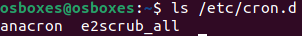
\includegraphics[width=12cm]{sch_sc_stealth_file_after.png}
	\caption{Listing files and directories at the cron.d directory after rootkit installation.}
	\label{fig:sc_stealth_file_after}
\end{figure}


\section{Rootkit persistence}
The files at \textit{/etc/cron.d} and \textit{/etc/sudoers.d} ensure the persistence of the rootkit in the infected system. As we explained in Section \ref{section:persistence}, these files are created by the \textit{deployer.sh} script before loading the rootkit. In this script, two constants define the contents of the entry written in these directories, as shown in Table \ref{table:rootkit_persistence_config}.

\begin{table}[htbp]
\begin{tabular}{|>{\centering\arraybackslash}p{3cm}|>{\centering\arraybackslash}p{4.5cm}|>{\centering\arraybackslash}p{6cm}|}
\hline
\textbf{FILENAME} & \textbf{CONSTANT} & \textbf{DESCRIPTION}\\
\hline
\hline
src/helpers/ deployer.sh & CRON\_PERSIST & Cron job to execute after reboot.\\
\hline
src/helpers/ deployer.sh & SUDO\_PERSIST & Sudo entry to grant password-less privileges.\\
\hline
\end{tabular}
\caption{Rootkit persistence module configuration.}
\label{table:rootkit_persistence_config}
\end{table}

Once the \textit{deployer.sh} script is excuted, the files are created  and, from that point onwards, the cron system will install the rootkit if it is not installed already once every minute. Table \ref{table:rootkit_persistence_config_defaults} shows the values of the configuration that must be set for user "osboxes". If the user of the infected system was another, or the script was located in a different location, the name of this user shall be changed.

\begin{table}[htbp]
\begin{tabular}{|>{\centering\arraybackslash}p{3cm}|>{\centering\arraybackslash}p{4.5cm}|>{\centering\arraybackslash}p{6cm}|}
\hline
\textbf{FILENAME} & \textbf{CONSTANT} & \textbf{VALUE}\\
\hline
\hline
src/helpers/ deployer.sh & CRON\_PERSIST & "* * * * * osboxes /bin/sudo /home/osboxes/TFG/apps/deployer.sh"\\
\hline
src/helpers/ deployer.sh & SUDO\_PERSIST & "osboxes ALL=(ALL:ALL) NOPASSWD:ALL \#"\\
\hline
\end{tabular}
\caption{Configuration for rootkit persistence module with the user "osboxes".}
\label{table:rootkit_persistence_config_defaults}
\end{table}



\section{Takeaways}
In the previous sections, we have explained the steps needed for using the different rootkit modules and displayed its functionalities in a test environment. As we saw, we were able to build at least one rootkit-like functionality using each of the capabilities we proposed at the beginning of this research work for our rootkit. As a summary, for each of these capabilities, we achieved the following:
\begin{itemize}
\item For hijacking running programs, we built a library injection mechanism that does not crash the process and thus allows for stealthy execution of code. We also incorporated a remote control capability for the malicious injected library so that we could execute commands remotely from the rootkit client.
\item With respect to backdoor and C2 capabilities we seeked for the rootkit, we built a comprehensive C2 system supporting multiple stealthy backdoor triggers and encrypted communication systems that allow for executing commands using the rootkit client, apart from an advanced method for exfiltrating data by modifying the outgoing traffic. The multiple stealthy features, as we explained in Section \ref{subsection:triggers}, allow for hiding data from network monitoring software using multiple techniques. Also, we demonstrated the backdoor capabilities for receiving and transmitting actions that manipulate the state of eBPF programs.
\item In the context of manipulating system calls, this was a key capability used in multiple of the rootkit modules. We were able to hijack the execution of programs or modify the contents of critical files in the system, such as \textit{/etc/sudoers}, which granted any rootkit user program privileged permissions.
\item With respect to rootkit persistence, we built a system that allows for surviving reboots, not only ensuring that the rootkit will be installed after one of these events, but also that the root permissions that were once granted to the rootkit the first time it was installed are maintained across reboots.
\item The stealth module we incorporated allows for hiding the directory where the rootkit is stored form the user, along with those files responsible from ensuring the rootkit persistence.
\end{itemize}

Taking into account all the above, we can confidently claim that we fulfilled the project objectives of our rootkit development.
